% !TeX spellcheck = en_GB
\documentclass[a4paper,12pt]{article}

\usepackage{anysize}
\marginsize{30mm}{20mm}{20mm}{20mm}
\usepackage[utf8]{inputenc}
\usepackage[english]{babel}
\usepackage[style=ieee,backend=biber,sorting=none]{biblatex}
\addbibresource{FinalReport.bib}
\usepackage{amsmath}
\usepackage{graphicx}
\graphicspath{ {./generatedImages/} }
\usepackage{svg}
\usepackage{setspace}
\singlespacing
\usepackage{gensymb}
\parskip 0ex 
\usepackage{array}
\newcolumntype{L}{>{\centering\arraybackslash}m{100mm}}
\newcolumntype{M}{>{\centering\arraybackslash}m{50mm}}
\newcolumntype{S}{>{\centering\arraybackslash}m{20mm}}


%opening
\title{Linear Direct Current Electromagnetic Motor with Liquid Eutectic Gallium-Indium Alloy Coil}
\author{Jason Guan}
\date{27 September 2019}
\begin{document}
\maketitle
\begin{center}
	892594255\\
	Department of Engineering Science\\
	Supervised by Dr. Bryan Ruddy
\end{center}

\newpage

\begin{abstract}
Abstract placeholder
\end{abstract}

\newpage

\section*{Acknowledgements}
Paul Roberts 

Steve Oldman 

Greg 

Nick, Suroosh, Mahsa and Yahya 

And of course, Dr. Bryan Ruddy 

\newpage

\tableofcontents

\newpage

\section{Table of Notation}
\begin{center}
	\begin{tabular}{c | L | c} 
		\textbf{Symbol} & \textbf{Description} & \textbf{Units} \\ [0.5ex] 
		\hline\hline
		$P_{in}$ & Electrical power input & $W$ \\ 
		\hline
		$P_{out}$ & Total power output & $W$ \\ 
		\hline
		$P_{mech}$ & Mechanical power output & $W$ \\ 
		\hline
		$P_{heat}$ & Heat power output & $W$ \\ 
		\hline
		$f$ & Frequency & $Hz$ \\ 
		\hline
		$\mathcal{F}$ & Magnetomotive force & $A$ \\ 
		\hline
		$\mathcal{R}$ & Magnetic reluctance & $H^{-1}$ \\ 
		\hline
		$\mathcal{R}_{mag}$ & Magnetic reluctance of the magnet & $H^{-1}$ \\ 
		\hline
		$\Phi$ & Magnetic flux & $Wb$ \\ 
		\hline
		$\Phi_0$ & Short circuit magnetic flux, i.e. flux in circuit when poles of magnet are connected with minimal reluctance & $Wb$ \\ 
		\hline
		$L_{Wtotal}$ & Total length of wire in motor & $m$ \\
		\hline
		$L_{mag}$ & Axial length of cylindrical magnet & $m$ \\
		\hline
		$B$ & Magnetic field density & $T$ \\
		\hline
		$B_{r}$ & Residual flux density of magnet & $T$ \\
		\hline
		$I$ & Electric current & $A$ \\
		\hline
		$d_{travel}$ & Required travel distance of the motor bobbin & $m$ \\
		\hline
		$c_{pWire}$ & Specific heat capacity of wire & $JKg^{-1}K^{-1}$ \\
		\hline
		$\mu_0$ & Vaccum permeability, $4\pi\times10^{-7} Hm^{-1}$ \cite{engineeringtoolboxPermeability2016} & $Hm^{-1}$ \\
		\hline
		$\mu_s$ & Relative magnetic permeability of mild steel, 760 \cite{baartmanMaterialsLibraryFEMM2007} & NA \\
		\hline
		$\mu_m$ & Relative magnetic permeability of neodymium magnet, 1.05 \cite{engineeringtoolboxPermeability2016} & NA \\
		\hline
	\end{tabular}
\end{center}

\newpage

\section{Introduction}

Soft robotics has in recent years enjoyed a surge in research interest. Traditional robots that use rigid materials for actuation tend to have poor adaptability and low human friendliness. Robots and actuators made with mechanically compliant materials may emerge more adaptable in unpredictable conditions and more comfortable for wearable use. 

Current soft robot actuation methods include chemical, pressure-based (pneumatic or hydraulic) and electroactive elastomer. Electromagnetic actuation that most traditional robots rely on has been mostly overlooked. Only four years ago, Jin et al. published \cite{jinStretchableLoudspeakerUsing2015}, the first paper that explored the idea. Jin introduced a voice coil speaker effective under large deformations. 

As a result, there is an opportunity add to the under-researched area of electromagnetic actuation for soft robots. Rigid electromagnetic actuation is a relatively mature field with a large existing corpus. 

Previously, electromagnetic actuation in soft robots was hindered by a lack of good conductors that maintain electrical properties under large deformations. Eutectic Gallium-Indium alloys (eGaIn) have emerged as a potential solution. eGaIn is a family of alloys that contain gallium, indium and sometimes tin and other metals. A typical eGaIn alloy can have 75\% Ga and 25\% In and melts at 15.5 \degree C \cite{dickeyEutecticGalliumIndiumEGaIn2008}, meaning it is liquid under room temperature. Liquid metal conductors can deform without large changes to material properties and do not undergo strain hardening or fatigue.

eGaIn is also advantageous among other liquid metals in that it has low toxicity \cite{dickeyEutecticGalliumIndiumEGaIn2008}, compared to mercury which is highly toxic. eGaIn is also stable in atmospheric conditions, compared to sodium-potassium alloy which is pyrophoric \cite{houghtonHazards2007}, and has low vapour pressure. eGaIn does however form an oxide layer on contact with oxygen which hinders its fluid and electrical properties \cite{liuCharacterizationNontoxicLiquidMetal2012}.

Using liquid metal in electromagnetic actuator coils also makes available a novel approach to cooling. The conductors themselves can be circulated and cooled externally, away from the rest of an actuator. This means that thermoregulation features such as cooling fins may become detached from the actuator, allowing for more compact designs where space is at a premium.

This project seeks to answer whether it is feasible to build an electromagnetic motor using liquid metal for wiring that can also be cooled via circulating metal in the wiring. To that end, an electromagnetic motor with eGaIn coils was designed, built and characterised. An analysis will also be conducted on whether eGaIn actuators hold promise for use in soft robots or for novel cooling approaches. 

\newpage

\section{Design, Manufacturing and Assembly}
\subsection{Mathematical Modelling}
\subsubsection{Motor Force}

\begin{equation} \label{eq:emmfdef}
\mathcal{F}=\mathcal{R} \Phi
\end{equation}
Magnetomotive force of a magnet can be calculated using total magnetic reluctance in a magnetic circuit and magnetic flux in that circuit, seen in equation \ref{eq:emmfdef}. This is analogous to electrical circuits following Ohm's law: magnetomotive force is analogous to voltage, reluctance is analogous to resistance and flux is analogous to current. Magnetomotive force in cylindrical magnets can be calculated using a short circuit scenario, i.e. by assuming poles of magnet are connected with minimal reluctance. Under the assumption that magnetic field density is uniform, the short circuit flux is equal to the remanence field density of the magnet multiplied by the cross-sectional area of the magnet normal to the direction of the magnetic field. In the case of an axially magnetised cylindrical magnet, this area is equal to the radial cross-section area of the cylinder.
\begin{equation}\label{eq:shortflux}
\Phi_0 = B_rA_{mag}
\end{equation}
Substituting equation \ref{eq:shortflux} into equation \ref{eq:emmfdef} gives a way to simply calculate $\mathcal{F}$ using axial length of magnet and remanent field density:
\begin{equation}\label{eq:emmf1}
\begin{split}
\mathcal{F} & = \mathcal{R}_{mag} \Phi_0\\
& = \frac{L_{mag}}{A_{mag}}B_r A_{mag}\\
& = L_{mag} B_r
\end{split}
\end{equation}
The magnetic circuit of a voice coil motor travels through four components in series: the magnet, the core, the "air" gap where the coils are and the shell, seen in figure \ref{fg:simplemotor}.
\begin{figure}[h!] 
	\centering
	\includegraphics[scale=0.4]{simplifiedMotor.png}
	\caption{Simplified axisymmetric diagram of typical moving-wire voice coil motor}
	\label{fg:simplemotor}
\end{figure}
This means the total reluctance in the circuit can be represented by equation \ref{eq:rttl}, similar to how resistance is calculated in an electrical circuit.
\begin{equation}\label{eq:rttl}
\mathcal{R}_{total}=\mathcal{R}_{gap}+\mathcal{R}_{mag}+\mathcal{R}_{core}+\mathcal{R}_{shell}
\end{equation}
Magnetic reluctance can be calculated as the proportion of magnetic path length $l_m$ and the product of material permeability $\mu$ and cross-sectional area normal to magnetic flux $A$, seen in equation \ref{eq:rcalc} \cite{coatesTransformerCoresReluctance2018}.
\begin{equation}\label{eq:rcalc}
\mathcal{R}=\frac{l_m}{\mu A}
\end{equation}
Assuming the shell and core are made out of magnetically conductive material such as mild steel, the permeability of shell and core will be hundreds of times higher than the permeability of "air" gap and magnet \cite{engineeringtoolboxPermeability2016}. Therefore, the reluctance of shell and core can be approximated to zero for the purposes of this calculation. 
Substituting simplified equation \ref{eq:rttl} into equation \ref{eq:emmfdef} produces:
\begin{equation}\label{eq:emmfreal}
\mathcal{F}=(\mathcal{R}_{gap}+\mathcal{R}_{mag})\Phi
\end{equation}
Reluctance between two coaxial cylinders, in this case between the magnet and the shell, can be calculated as in equation \ref{eq:rgap}, assuming all magnetic flux flows through the core \cite{changChapterElectrodynamics2006}. Relative permeability of the gap is approximated to 1 as none of air, silicone or eGaIn are ferromagnetic \cite{engineeringtoolboxPermeability2016}.
\begin{equation}\label{eq:rgap}
\mathcal{R}_{gap}=\frac{\mu_0 \ln{\frac{r_{out}}{r_{in}}}}{2\pi L_{core}}
\end{equation}
Reluctance through the magnet can be calculated as seen in equation \ref{eq:rmag}, similar to how resistance would be calculated for a cylinder.
\begin{equation}\label{eq:rmag}
\mathcal{R}_{mag}=\frac{\mu_m L_{mag}}{2\pi r_{mag}^2}
\end{equation}
Substituting equations \ref{eq:rgap}, \ref{eq:rmag} and \ref{eq:emmf1} into equation \ref{eq:emmfreal} gives equation \ref{eq:emmfsubbed} which yields flux in the motor magnetic circuit.
\begin{equation}\label{eq:emmfsubbed}
\begin{split}
L_m B_r & = \frac{\ln{\frac{r_{out}}{r_{in}}}}{2\pi L_c}\Phi\\
\frac{2\pi L_m L_c B_r}{\ln{\frac{r_{out}}{r_{in}}}} & = \Phi\\
\end{split}
\end{equation}
To calculate the magnetic field density in the "air" gap, which can then be used to calculate force acting on the moving coils, the area of action that the flux is distributed across is also required as seen in equation \ref{eq:fluxdef}.
\begin{equation}\label{eq:fluxdef}
\Phi = B_{gap}A_{active}
\end{equation}
Substituting equation \ref{eq:fluxdef} into equation \ref{eq:emmfsubbed} gives equation \ref{eq:fluxsubbed}, which can be used to calculate the magnetic field density $B_{gap}$ across the "air" gap.
\begin{equation}\label{eq:fluxsubbed}
B_{gap} = \frac{2\pi L_{mag} L_{core} B_r}{\ln{\frac{r_{out}}{r_{in}}}A_{active}}
\end{equation}
Using Lorentz's force law substituted with equation \ref{eq:fluxsubbed}, equation \ref{eq:fbil} gives a minimum current $I$ can be obtained given a known required force $F$ and a known length of wire i
n the magnetic field $L_{active}$.
\begin{equation}\label{eq:fbil}
\begin{split}
F & = B_{gap}IL_{active}\\
I & = \frac{F}{B_{gap}L_{active}}\\
I & = \frac{F A_{active} \ln{\frac{r_{out}}{r_{in}}}}{2\pi L_{mag} L_{core} B_r L_{active}}
\end{split}
\end{equation}
The active area in the magnetic field is different for each layer of wire in the motor. Layers of wire further away from the magnet, meaning a larger area and therefore lower magnetic field density. The total active area that magnetic flux is distributed across can be calculated as shown in equation \ref{eq:activearea}, where $n$ is the total number of wire layers.
\begin{equation}\label{eq:activearea}
A_{active} = \sum_{1}^{n}{A_{active}^{layer}} = 2\pi L_c (r_{core}-r_{wireout} + 2r_{wireout} \frac{(n+1)n}{2})
\end{equation}
The length of wire in the magnetic field can be calculated in a similar fashion, shown in equation \ref{eq:activel}.
\begin{equation}\label{eq:activel}
L_{active} = L_{core}\pi(layers+1)layers + \frac{L_{core} r_{mag} \pi}{r_{wireOut}}
\end{equation}
Combining equations \ref{eq:fbil}, \ref{eq:activearea} and \ref{eq:activel} yields a final current calculation seen in equation \ref{eq:finalcurrent}.
\begin{equation}\label{eq:finalcurrent}
I = \frac{F\cdot 2\pi L_c (r_{core}-r_{wireout} + 2r_{wireout} \frac{(n+1)n}{2}) \ln{\frac{r_{out}}{r_{in}}}}{2\pi L_{mag} L_{core} B_r L_{core}\pi(layers+1)layers + \frac{L_{core} r_{mag} \pi}{r_{wireOut}}}
\end{equation}

\subsubsection{Heat and Temperature}
A major challenge for designing electromagnetic motors is coil heat generation, and how to dissipate that heat. Energy is conserved in the motor system, as seen in figure \ref{fg:motorheat} and equation \ref{eq:pbreakdown}. As a result,  

\begin{figure}[h!]
\centering
\includegraphics[scale=0.4]{motorheat.png}
\caption{Conservation of energy in the motor system}
\label{fg:motorheat}
\end{figure}
\begin{equation}\label{eq:pbreakdown}
P_{in}=P_{out}=P_{mech}+P_{heat}
\end{equation}

\begin{equation}\label{eq:pin}
P_{in} = IV = I^2R
\end{equation}

\begin{equation}\label{eq:resistance}
R=\frac{L_{Wtotal}}{A\sigma}
\end{equation}

\begin{equation}\label{eq:pmechbreakdown}
\begin{split}
P_{mech} & = \vec{F}\vec{d}\\
& = BIL\cdot d_{travel} \cdot f
\end{split}
\end{equation}

Combining equations \ref{eq:pin}, \ref{eq:resistance}, \ref{eq:pbreakdown} and \ref{eq:pmechbreakdown} gives a formulation for temperature change of wires, assuming heat energy is conserved in wires:

\begin{equation}\label{eq:pheatbreakdown}
\begin{split}
P_{heat} & = P_{in}-P_{mech}\\
\rho Q c_{pWire} \Delta T & = \frac{I^2L_{Wtotal}}{A\sigma}-BIL\cdot d \cdot f \\
\Delta T & = \frac{\frac{I^2L_{Wtotal}}{A\sigma}-BIL\cdot d \cdot f}{\rho Q c_{pWire}}
\end{split}
\end{equation}


\subsection{Optimisation Algorithm}
\begin{figure}[h!] 
	\centering
	\includegraphics[scale=0.4]{optiAlgro.png}
	\caption{Diagrammatic representation of optimisation algorithm inputs and outputs}
	\label{fg:optiAlgo}
\end{figure}

Grid-search optimisation for even numbered layers.

\begin{table} [h!] 
	\centering
	\caption{Grid-search optimisation variables and units.}
	\label{tb:gridsearch}
	\begin{tabular}{c | c} 
		\textbf{Variable} & \textbf{Units} \\ [0.5ex] 
		\hline\hline
		Magnet length & m \\
		\hline
		Magnet radius & m \\
		\hline
		Core length & m \\ 
		\hline
		Bobbin length & m \\
	\end{tabular}
\end{table}

Optimised for an optimisation variable $\mathcal{P}$, which is the product of total motor mass and electrical input power.

Runs requirement checking function on each result and discards invalid solutions.

\begin{table} [h!] 
	\centering
	\caption{List of optimisation requirements and justifications.}
	\label{tb:optrequirements}
	\begin{tabular}{M | M | M} 
		\textbf{Variable} & \textbf{Requirement} & \textbf{Justification} \\ [0.5ex] 
		\hline\hline
		Output force & Must be over 9 N & Minimum to drive liquid metal pump \\
		\hline
		Acceptable temperature change in wires after circulation & Must be under 30 K & Higher temperatures may be a health and safety hazard \\
		\hline
		Travel distance of motor & Must be over 9 mm & Minimum to drive liquid metal pump \\ 
		\hline
		Bobbin length & Must be shorter than combined length of core and magnet & Not physically valid otherwise \\ 
		\hline
		Shell internal diameter & Must be under 80 mm & Not practical for manufacturing, assembly and handling if bigger \\ 
		\hline
		Total motor current & Must be under 10 A & No power supply available to drive more than 10 A \\ 
		\hline
		Total volume of wire & Must be under 15 ml & Limit to amount of eGaIn available and difficult to assemble with larger volume \\ 
		\hline
		Flow rate of liquid metal in wires & Must be positive & Validity check \\ 
		\hline
		Electrical power input & Must be positive & Validity check \\ 
		\hline
	\end{tabular}
\end{table}

Optimisation was conducted assuming the use of 2 mm internal diameter, 3 mm external diameter silicone tubing for wiring. This was the tubing with largest internal volume to total volume ratio that was commercially available.

The optimisation software produced physical dimensions, pump flow and pressure requirements, electrical input requirements and an axisymmetric cross-section diagram to show scale of the optimised motor for each number of layers that the optimisation was run for.

\begin{table} [h!]
	\centering
	\caption{Comparison between most efficient 4-layer and 6-layer motor designs.}
	\label{tb:optoutput}
	\begin{tabular}{M | c | c | c} 
		\textbf{Variable} & \textbf{4-layer solution} & \textbf{6-layer solution} & \textbf{Units} \\ [0.5ex] 
		\hline\hline
		Magnet length & 35 & 42.5 & $mm$ \\ 
		\hline
		Magnet radius & 20 & 20 & $mm$ \\ 
		\hline
		Core length & 12 & 8 & $mm$ \\ 
		\hline
		Bobbin length & 27.5 & 23.75 & $mm$ \\ 
		\hline
		Shell internal radius & 33.5 & 39.5 & $mm$ \\ 
		\hline
		Total wire length & 6.68 & 9.55& $m$ \\ 
		\hline
		Total wire resistance & 0.15 & 0.22 & $\Omega$ \\ 
		\hline
		Minimum required current & 7.75 & 6.27 & $A$ \\ 
		\hline
		Minimum required voltage & 1.19 & 1.38 & $V$ \\ 
		\hline
		Minimum power input & 9.22 & 8.63 & $W$ \\ 
		\hline
		Flow rate required for circulation cooling & 0.135 & 0.125 & $ml\cdot s^{-1}$ \\ 
		\hline
		Pressure required to drive circulation cooling & 5.51 & 7.28 & $kPa$ \\ 
		\hline
		Total mass of motor & 1.21 & 1.50 & $kg$ \\ 
		\hline
		Optimisation Variable $\mathcal{P}$ & 11.19 & 12.98 & $kg\cdot W$ \\ 
		\hline
	\end{tabular}
\end{table}

Choice between 4 layer design and 6 layer design

\begin{figure}[h!] 
	\centering
	\includegraphics[width=0.5\textwidth]{finalDesign_layers.png}
	\caption{Cross-section diagram of final motor design}
	\label{fg:finalmotor}
\end{figure}

\subsection{Design Validation}
ANSYS Maxwell 2D electromagnetic simulation, axisymmetric about z-axis.
\begin{figure}[h!] 
	\centering
	\includegraphics[width=0.5\textwidth]{maxwell.png}
	\caption{Maxwell 2D simulation of magnetic field density in motor}
	\label{fg:maxwellB}
\end{figure}

\begin{figure}[h!] 
	\centering
	\includegraphics[width=\textwidth]{force.png}
	\caption{Convergence of force on wires to 9.0882 N in Maxwell 2D simulation}
	\label{fg:maxwellforce}
\end{figure}

\subsection{Physical Design and Manufacturing}
4 axial, 40 mm diameter, 10 mm tall N45 grade neodymium disc magnets were used in series, to substitute for the required 40 mm diameter, 42.5 mm tall N42 grade neodymium magnet. The disc magnets also come with countersunk unthreaded M6 holes for fastening. 

\subsubsection{Shell}
Two-piece design, cylinder and base
To enable safe assembly of magnets into motor
M6 threads at centre of base to secure magnets and core
Holes at end to secure spacer, and also enable ventilation while motor is in operation
M3 threaded holes in side to secure shell cylinder during assembly step that attaches base, magnets and core to cylinder.
Both turned on lathe from 1020 grade 100 mm diameter engineering bar steel stock

\begin{figure}[h!] 
	\centering
	\includegraphics[scale=0.5]{shellcylinder.png}
	\caption{Axisymmetric cross-section drawing of final shell cylinder}
	\label{fg:shellcylinder}
\end{figure}

\begin{figure}[h!] 
	\centering
	\includegraphics[scale=0.5]{shellbase.png}
	\caption{Axisymmetric cross-section drawing of final shell base. Units in mm.}
	\label{fg:shellbase}
\end{figure}

\subsubsection{Core}
8 mm thick, 40 mm diameter cylinder with countersunk unthreaded M6 hole in the centre. A bolt travels through the hole that secures the core to the magnets to the shell base. 

\begin{figure}[h!] 
	\centering
	\includegraphics[scale=0.5]{core.png}
	\caption{Axisymmetric cross-section drawing of final core. Units in mm.}
	\label{fg:core}
\end{figure}

\subsubsection{Wire Bobbin}

\begin{figure}[h!] 
	\centering
	\includegraphics[scale=0.5]{bobbin.png}
	\caption{Three-view drawing of final wire bobbin. Units in mm.}
	\label{fg:bobbin}
\end{figure}

\subsection{Assembly}

\subsubsection{Shell and Magnet Assembly}
\begin{figure}[h!] 
	\centering
	\includegraphics[width=0.5\textwidth]{placeholder.png}
	\caption{Contraption used to safely assemble magnets and core onto shell base.}
	\label{fg:assemblingmagnet}
\end{figure}

\begin{figure}[h!]
	\centering
	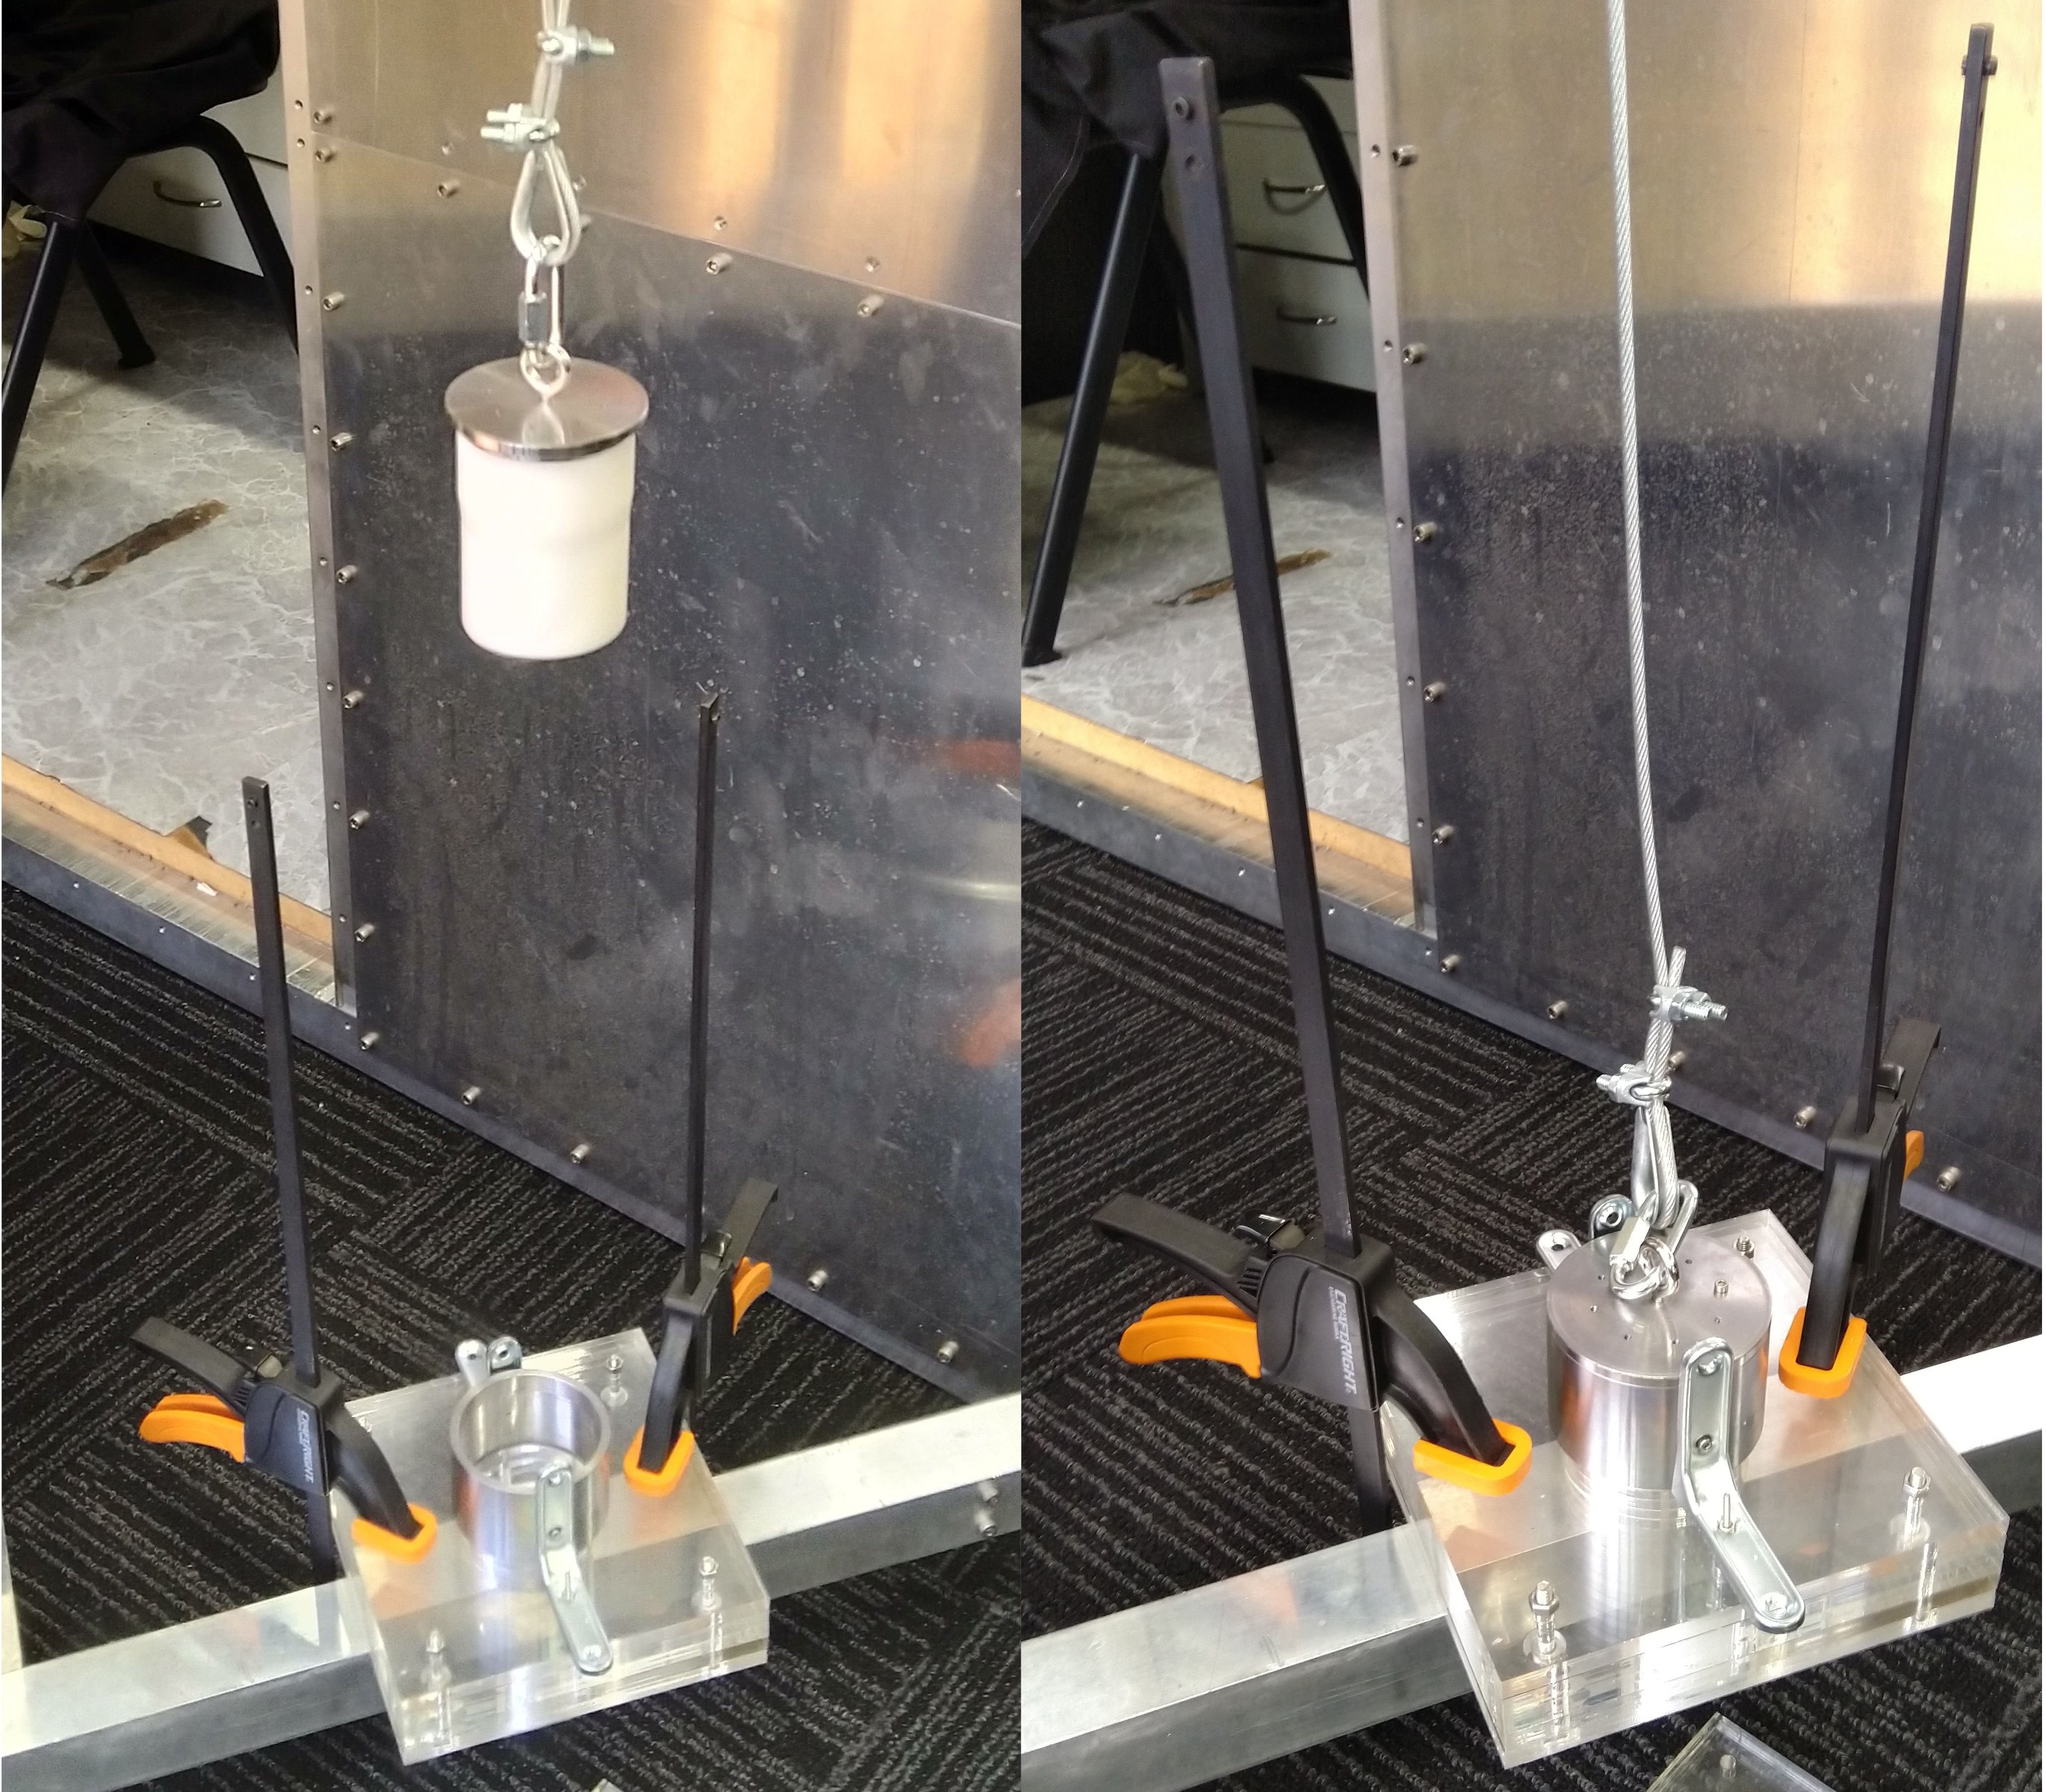
\includegraphics[width=0.5\textwidth]{assemblingshell.png}
	\caption{Shell base with magnets and core attached being lowered onto shell cylinder.}
	\label{fg:assemblingshell}
\end{figure}

\begin{figure}[h!]
	\centering
	\includegraphics[width=0.5\textwidth]{assembledshell.jpg}
	\caption{Assembled shell with magnets and core attached.}
	\label{fg:assembledshell}
\end{figure}

\subsubsection{Wire Assembly}
\begin{figure}[h!]
	\centering
	\includegraphics[width=0.5\textwidth]{assembledbobbin.jpg}
	\caption{Bobbin with complete silicone tube windings. Tubes wound by hand.}
	\label{fg:assembledbobbin}
\end{figure}

\subsubsection{Health, Safety and Containment}
Gallium, indium and eGaIn are not toxic to touch, but can cause harm if ingested or inhaled.

However, eGaIn is known to be corrosive towards most solid metals including iron, copper and aluminium alloys \cite{cuiLiquidMetalCorrosion2018}. In particular, without specific surface treatment, aluminium parts in the lab may corrode on contact with eGaIn.

Everything done in fish bin, done in a corner of the lab away from metal components that can be damaged.

To avoid accidental ingestion after handling eGaIn, disposable gloves were worn whenever there was possible exposure to eGaIn.

\newpage

\section{Experiment Designs and Results}

\subsection{Experiment 1: Force Characterisation}

\subsubsection{Method}
Plate on bobbin, motor oriented vertically. 

\begin{figure}[h!]
	\centering
	\includegraphics[width=0.3\textwidth]{placeholder.png}
	\caption{Experiment setup to characterise force output of motor given different electrical input.}
	\label{fg:forceexperiment}
\end{figure}

\subsubsection{Results}

\begin{figure}[h!]
	\centering
	\includegraphics[width=\textwidth]{resultforcevcurrent.png}
	\caption{Experimental result motor force  plotted against provided current.}
	\label{fg:forceplot}
\end{figure}


\begin{table}[h!] 
	\centering
	\caption{Analysis of force experiment results.}
	\label{tb:fullresults3}
	\begin{tabular}{ lll }
		Item & Value & Units \\
		\hline\hline
		Average efficiency ex. Bobbin & 1.00 & $NA^{-1}$ \\
		\hline
		Mass of bobbin \& fixed cup & 335.22 & g \\
		\hline
		Current required for 9 N & 8.75 & A \\
		\hline
		Theoretical current for 9 N & 8.50 & A \\
		\hline 
	\end{tabular}
\end{table}

\subsection{Experiment 2: Circulation Thermoregulation}

\subsubsection{Method}

\subsubsection{Results}

\newpage

\section{Discussion}

Application to the original physical situation\\ 

Comparison with related problems and other solutions\\

If the eGaIn in the final motor design was substituted for copper threaded through silicone tubing, the motor would require much less power to produce the same force output. A motor of the same size filled with copper coils of the same diameter instead of eGaIn will consume under half of the power for the same force output. If the volume of the wiring was substituted entirely for 0.22 mm diameter copper wire, a common type of wire used for electromagnetic motors of this force scale, the motor would draw ~18 times less power to produce the same force.
\begin{table}[h!]
	\centering
	\caption{Comparison between final eGaIn motor and two hypothetical solutions using copper wiring.}
	\label{tb:coppercompare}
	\begin{tabular}{M | c | c | c | c} 
		\textbf{Variable} & \textbf{eGaIn solution} & \textbf{Copper equal} & \textbf{Copper fill} & \textbf{Units} \\ [0.5ex] 
		\hline\hline
		Total wire length & 9.55 & 9.55 & 157.76 & $m$ \\ 
		\hline
		Total wire resistance & 0.22 & 0.026 & 34.86 & $\Omega$ \\ 
		\hline
		Required current & 6.27 & 6.27 & 0.12 & $A$ \\ 
		\hline
		Power input & 8.63 & 3.12 & 0.46 & $W$ \\ 
		\hline
	\end{tabular}
\end{table}

Critical assessment of significance\\

Difficulty of the problem and how well it has been tackled\\

\newpage

\section{Conclusion}

\newpage

\section{Appendices}
\subsection{Full Results of Motor Force Experiment}
\begin{table}[h!]
	\centering
	\caption{Results from motor force experiment.}
	\label{tb:fullresults1}
	\begin{tabular}{SSSSSSS}
		Number of Weights & Incremental Mass Balanced (g) & Total Mass Balanced (g) & Total Force (N) & Voltage (V) & Current (A) & Power (W)\\
		\hline\hline
		0 & 335.22$\dagger$ & 335.22 & 3.29 & 1.57 & 3.30 & 5.18\\
		\hline
		1 & 81.53 & 416.75 & 4.09 & 1.96 & 4.10 & 8.04 \\
		\hline
		2 & 81.11 & 497.86 & 4.88 & 2.36 & 5.00 & 11.80\\
		\hline
		3 & 81.32 & 579.18 & 5.68 & 2.72 & 5.70 & 15.50 \\
		\hline
		4 & 81.12 & 660.30 & 6.48 & 3.05 & 6.60 & 20.13 \\
		\hline
		5 & 81.65 & 741.95 & 7.28 & 3.45 & 7.60 & 26.22 \\
		\hline
		6 & 81.19 & 823.14 & 8.07 & 3.68 & 8.30 & 30.54 \\
		\hline
		7 & 81.43 & 904.57 & 8.87 & 4.07 & 9.30 & 37.85 \\
		\hline
		8 & 80.65 & 985.22 & 9.66 & 4.35 & 9.90 & 43.07 \\
		\hline
	\end{tabular}
	$\dagger$Estimated using average efficiency, seen in table \ref{tb:fullresults3} calculated from incremental current required to produce incremental force, both seen in table \ref{tb:fullresults2}.
\end{table}


\begin{table}[h!]
	\centering
	\caption{Incremental values between adding each additional weight during motor force experiment`.}
	\label{tb:fullresults2}
	\begin{tabular}{SSSS}
		Number of Weights & Force increment (N) & Current increment (A) & Incremental Efficiency (N/A) \\
		\hline\hline
		0 & 3.29 & 3.30 & 1.00 \\
		\hline
		1 & 0.80 & 0.80 & 1.00 \\
		\hline
		2 & 0.80 & 0.90 & 0.88 \\
		\hline
		3 & 0.80 & 0.70 & 1.14 \\
		\hline
		4 & 0.80 & 0.90 & 0.88 \\
		\hline
		5 & 0.80 & 1.00 & 0.80 \\
		\hline
		6 & 0.80 & 0.70 & 1.14 \\
		\hline
		7 & 0.80 & 1.00 & 0.80 \\
		\hline
		8 & 0.79 & 0.60 & 1.32 \\
		\hline
	\end{tabular}
\end{table}



\newpage
\printbibliography
	
\end{document}
